\chapter{Curse of the Abyss}

\section{Ascending the Abyss}
The abyss harbors a mysterious phenomenon known as the Curse of the Abyss. It manifests when delvers attempt to ascent the abyss. This curse makes ascending a daunting affair, resulting in exhaustion and distress, even for the most seasoned delver. The deeper you go ascend from the more severe the curse's effect will be. The illustrations show some of the curse's effects.

\subsection{Exhaustion Points}
{All delvers start their descent with 0 exhaustion points out of a maximum of 3.}

\subsection{Roll for Exhaustion (2d6)}
{Whenever a delver attempts to ascend a layer of the abyss they must make a (2d6) exhaustion check to determine how many exhaustion points they gain. On a 10 or higher, they gain (+0) exhaustion points, 9 to 7 they gain (+1) point of exhaustion, and on a 6 or lower they gain (+2) points of exhaustion. \newline Should a delver find themselves ascending from beyond their recommended layer they will take (-2) penalty to their roll.}

\subsection{Exhaustion Recovery}
{A delver can recover from this state by taking a long rest. A delver can subtract 1 exhaustion point for each long rest. A delver that reaches the city of Orth can recover all of their exhaustion points after a short rest.}

\subsection{Exhaustion Consequences}
{Should a delver's exhaustion point reach 3, the partial effects of a layer's curse will apply. An affected delver succumbs to their exhaustion - and is unable to move on their own nor perform any actions. They are in a constant state of drifting in and out of consciousness. \newline In the case that their exhaustion point should exceed 3 the effects of the curse will have its full effect on the delver. In the worst case scenario depending on the description of the curse the delver dies.}

%\begin{figure*}%[ht!]
\begin{center}
\begin{tabular}{cc}
\adjustbox{trim={.25\width} 0 {0.25\width} 0,clip}{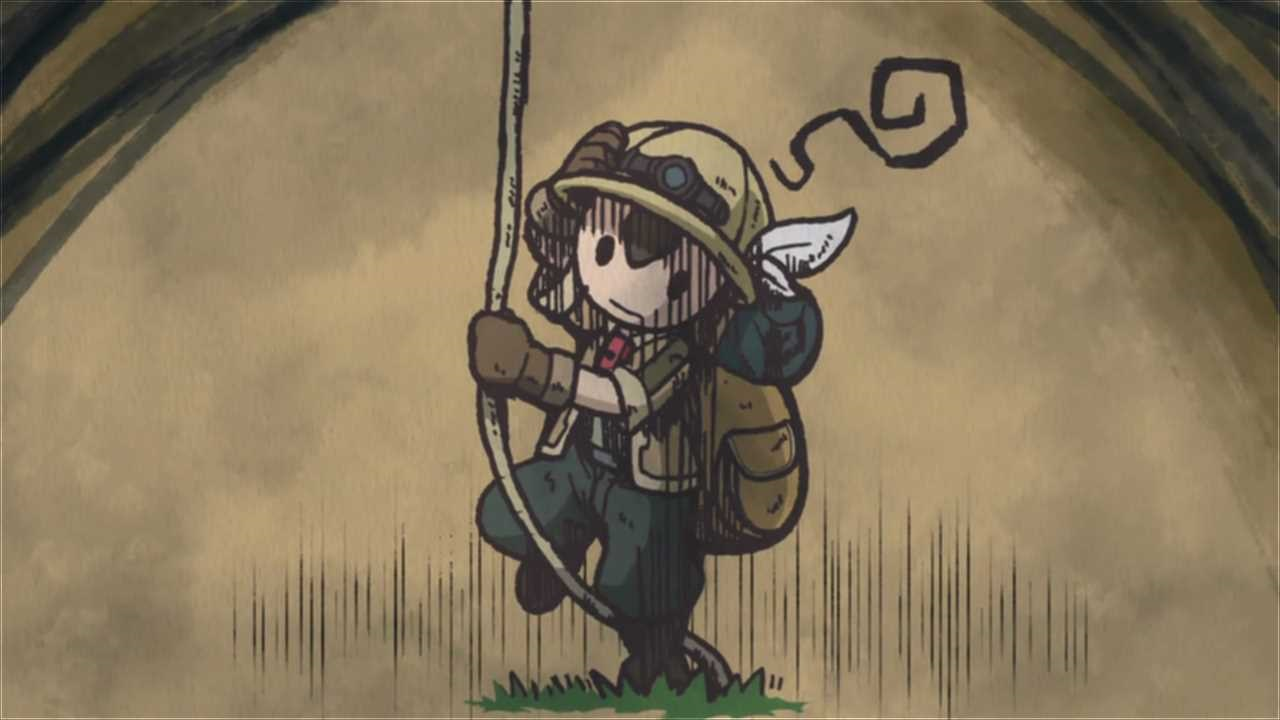
\includegraphics[width=7.3cm]{img/curses/1.png}} &
\adjustbox{trim={.25\width} 0 {0.25\width} 0,clip}{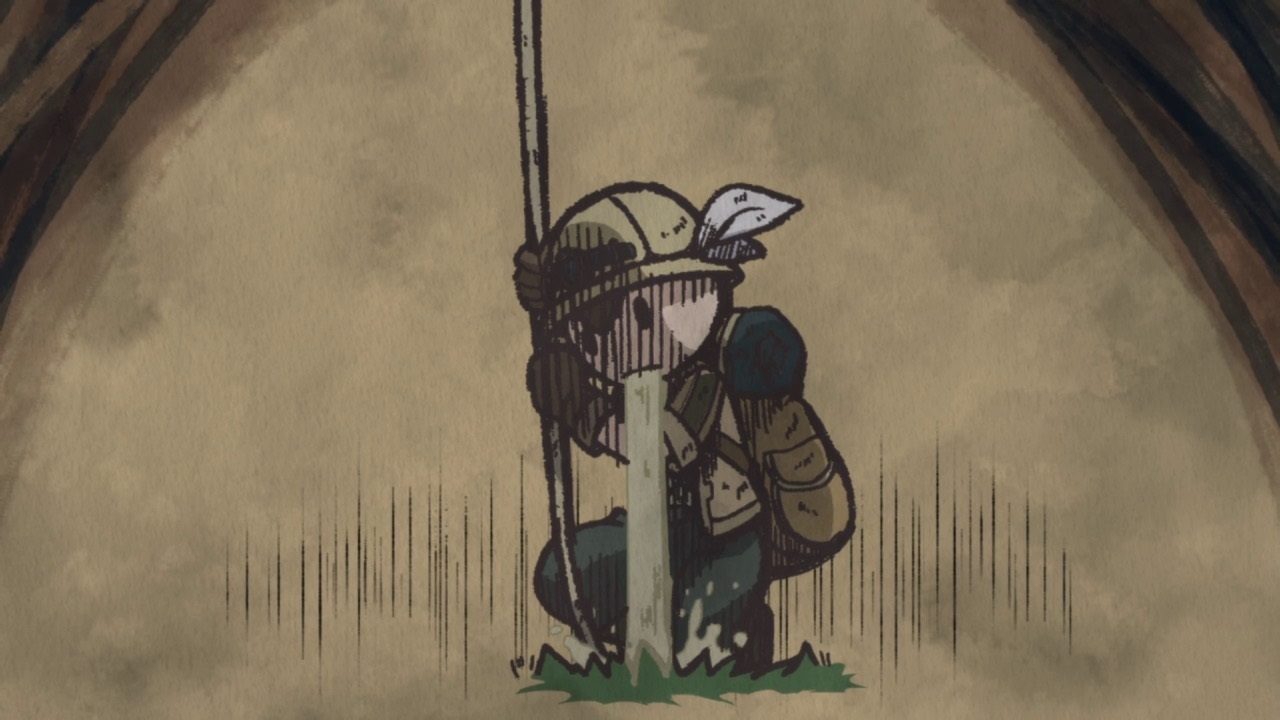
\includegraphics[width=7.3cm]{img/curses/2.png}} \\
 a) & b)\\
 \end{tabular}
\captionof{figure}{a) b) It is common for delvers who ascend from the 3rd to 1st layers to experience nausea, motion sickness, puking, and confusion.}
\end{center}
\begin{center}
\begin{tabular}{cc}
\adjustbox{trim={.25\width} 0 {0.25\width} 0,clip}{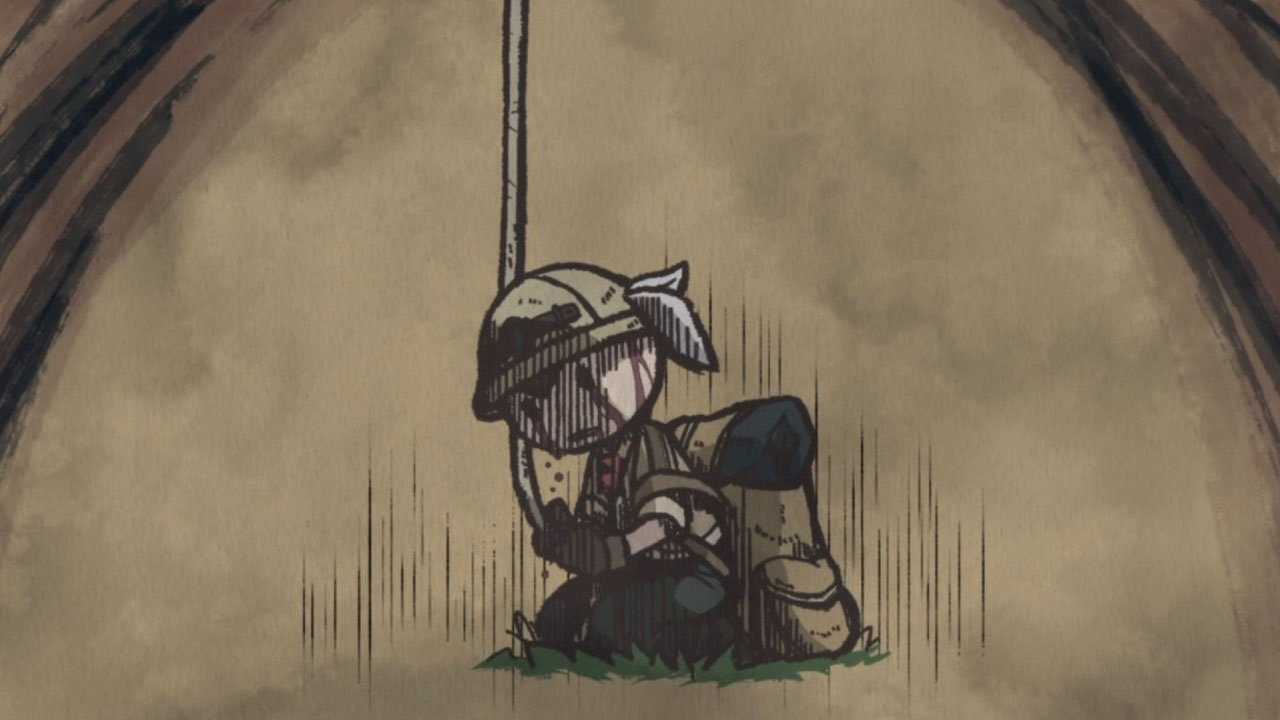
\includegraphics[width=7.3cm]{img/curses/4.png}} &
\adjustbox{trim={.25\width} 0 {0.25\width} 0,clip}{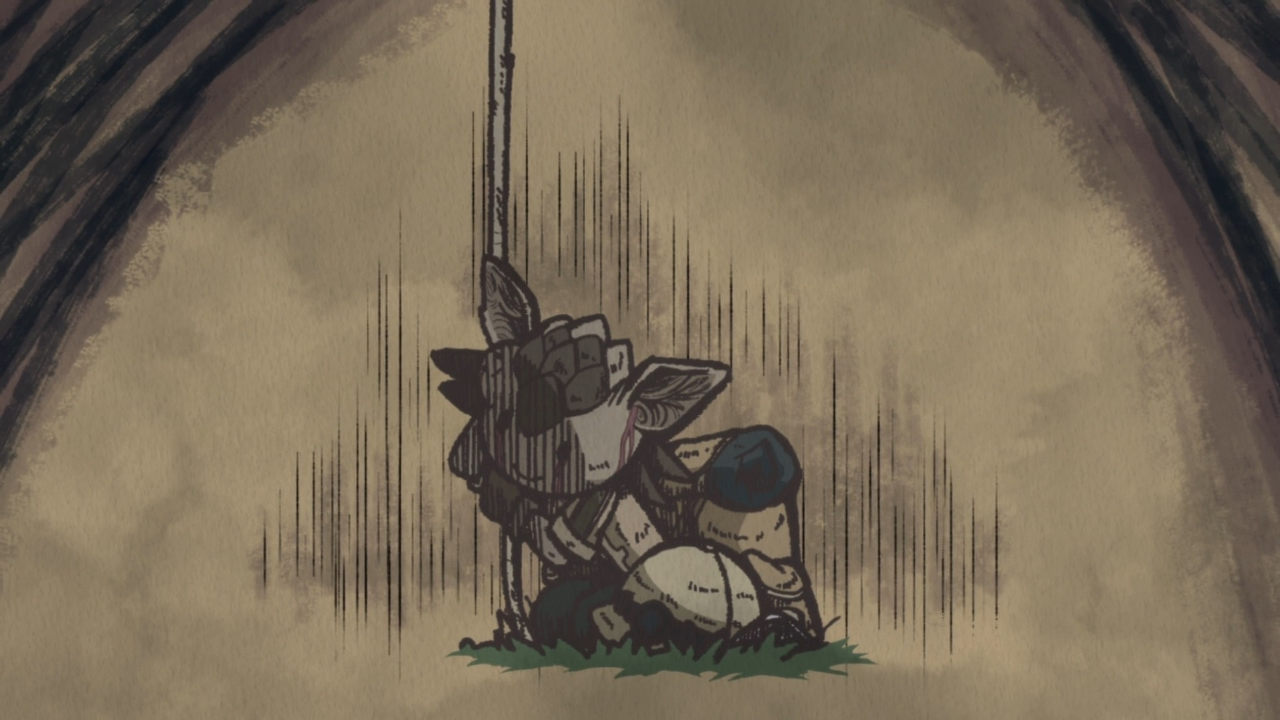
\includegraphics[width=7.3cm]{img/curses/5.png}} \\
 c) & d)\\
 \end{tabular}
\captionof{figure}{c) Delvers attempting to ascend from the 4th layer are exposed to severe hemorrhaging from all orifices. 5th layer results in intense pain and confusion resulting in self harm. d) 6th layer may result in loss of humanity. These curses can be deadly.}
\end{center}
\begin{center}
\begin{tabular}{c}
\adjustbox{trim={.1\width} 0 {0.1\width} {1cm},clip}{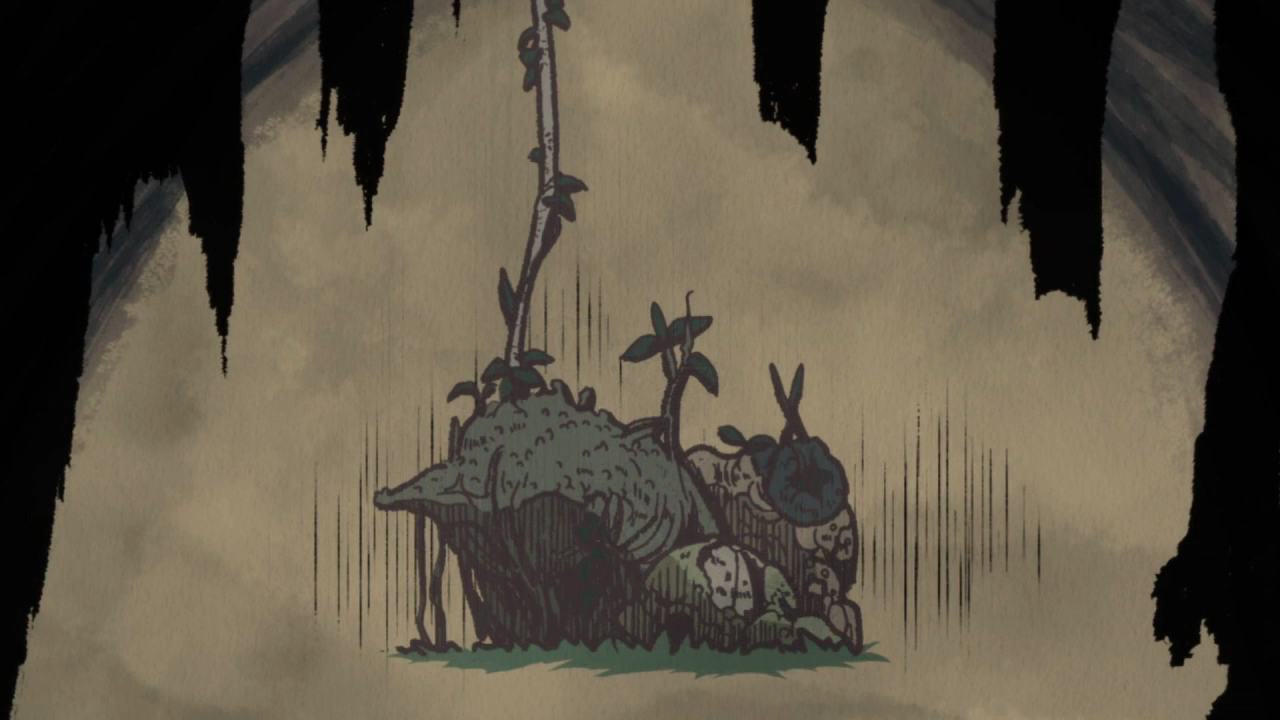
\includegraphics[width=9.5cm]{img/curses/6.png}} \\
 e)\\
 \end{tabular}
\captionof{figure}{e) Descending into the 6th layer is known as the Last Dive. Curses beyond this point are severe and lethal for humans.}
\end{center}
%\end{figure*}

\section{Humanity}

You start with 10. The effects of a lack of humanity are complex and multi-faceted. Every failure you experience will reduce your humanity.

Whenever a person 

20: You are a well-adjusted, normal human being.
 19-15: You are worldly and have experienced hardship in your life, though you aren’t necessarily less moral or worse of a person because of that. 
15-13: Your life experiences have left you callous and shrewd, distant from others from the tragedies you have lived through. Still not necessarily bad, however.
13-10: Actual physical changes occur at this threshold, as the Abyss Curse changes one due to lack of Humanity. Small physical things, like needing to look through lenses to not get headaches, fingernails falling out and not regrowing, unnatural shortness despite genetics, lack of pigment in or persistently dry skin are all symptoms of this. No mental changes, still.
10-8: Marked mental and physical changes occur. One’s own sense of sight, smell and spatial awareness are enhanced. People exhibit clearly inhuman features at this stage: tar-black irises, extreme paleness, animal-like behaviour, a very loose grasp of morality, abnormal musculature, inability to be socially acceptable, and severe alterations of personality are all symptoms of this stage. Most White-Whistles sit in this range.
7-5: Treading an extremely fine line between human and monster, one’s physical abilities are once again increased, though at the detriment of their sanity and biology. A total inability to understand ethics, personal space, human rights or even basic dignity. Bones harden and become harder to break, though warp and shape themselves in ways that make uncanny changes to one’s body. One can only get to this point by repeated exposure to the Curse at the 5th layer or below, or the constant abuse of certain relics. While intelligence and willpower doesn’t suffer, victims at this stage often become unnaturally fixated on one goal at a time, and will single-mindedly pursue it even to their death.
4-2: Total loss of what makes one a human being. Most basic animals sit here. Ranging in mental ability from pack animals to slugs.
1-0: Inanimate objects, and things with only the most basic functions. Sponges, fungi, jellyfish, plants all make up this category.

